\documentclass[12pt]{article}

\usepackage[margin=1in]{geometry}
\usepackage{amsmath}
\usepackage{biblatex}
\usepackage{parskip}
\usepackage{graphicx}
\usepackage{float}
\usepackage{fancyhdr}
\usepackage{lastpage}
\usepackage{titlesec}
\usepackage{enumitem}
\usepackage{subfig}
\usepackage{hyperref}
\usepackage{soul}
\usepackage{color}
\usepackage{colortbl}

\pagestyle{fancy}
\renewcommand{\headrulewidth}{0pt}
\renewcommand{\footrulewidth}{0pt}
\fancyhf{}
\lfoot{\scriptsize January 2019}
\cfoot{\scriptsize Brendon Matusch---Improving Particle Classification in WIMP Experiments}
\rfoot{\scriptsize Page~\thepage~of~\pageref{LastPage}}

\graphicspath{{./images/}}

\addbibresource{paper.bib}

\titlespacing{\section}{0pt}{0pt}{0pt}
\titlespacing{\subsection}{0pt}{0pt}{0pt}
\titlespacing{\subsubsection}{0pt}{0pt}{0pt}

\titleformat*{\section}{\normalsize\bfseries}
\titleformat*{\subsection}{\normalsize\bfseries}
\titleformat*{\subsubsection}{\normalsize\bfseries}

\begin{document}

\begin{center}
    \begin{large}
        Improving Particle Classification in WIMP Dark Matter Detection Experiments Using Neural Networks -- Brendon Matusch
    \end{large}
\end{center}

\section{Introduction}

In all experiments for detection of WIMP dark matter, it is essential to develop a classifier that can distinguish potential WIMP events from background radiation. Most often, classifiers are developed manually, via physical modeling and empirical optimization. This is problematic for two reasons: it takes a great deal of time and effort away from developing the experiment, and the resulting classifiers often perform suboptimally (which means that a greater amount of expensive run time is required to obtain a confident experimental result).

Machine learning has the potential to automate this and accelerate experimentation, and also to detect patterns that humans cannot. However, two major challenges, which are shared among several dark matter experiments, stand in the way: impure calibration data, which hinders training of models, and unpredictable physical dynamics within the detector itself.

My objective was to develop a set of machine learning techniques that resolve these two problems, and thus more efficiently generate highly accurate classifiers.

I was able to obtain raw data for two dark matter experiments which exhibit these challenges: the PICO-60 bubble chamber \cite{pico}, and the DEAP-3600 liquid argon scintillator \cite{deap}.

In PICO-60, background alpha and WIMP-like neutron calibration datasets are used for training; however, there is an impurity of 10\% alphas in the neutron set. While a conventional classifier was developed (and is believed to be 100\% accurate), machine learning in the form of a supervised neural network (NN) has also been previously explored, because of the benefits of automation. Unfortunately, it achieved a mean accuracy of only 80.2\% -- not usable as a practical replacement for conventional methods in future iterations of the experiment.

In DEAP-3600, photons are absorbed and re-emitted by a wavelength shifting medium in an unpredictable direction, before being detected by one of 255 photomultiplier tubes (PMTs) arranged in a hexagonal lattice on the surface of the spherical detector. The unpredictability severely limits the accuracy of conventional classifiers; the best classifier so far removes 99.6\% of alpha background radiation, while also (undesirably) removing 91.0\% of WIMP events. Because of physical limitations, simulated data is used for calibration, with a limited amount of real-world experimental data available for testing.

I composed a 28-page research whitepaper \cite{me} about my work on PICO-60, which has been reviewed and approved by the PICO collaboration and pre-published at \url{https://arxiv.org/abs/1811.11308}. It is currently undergoing peer review for eventual publication in the journal \textit{Computer Physics Communications}.

\ul{All PICO researchers are listed on my paper for their work on the original PICO-60 experiment. They did not contribute to this study; I completed and documented it independently.}

\section{Procedure}

\subsection{Resolving Impurities (PICO-60)}

In the context of PICO-60, my intent was to develop a highly accurate classification algorithm that is tolerant to substantial impurities in calibration data. I developed and compared two sets of classification algorithms: supervised learning, and semi-supervised learning.

\subsubsection{Supervised Learning}

I experimented with supervised learning, exploring the following data formats to determine which facilitates the best-performing solution:

\begin{enumerate}
    \item An 8-band Fourier transform of audio recorded in the detector. I applied a dense NN with dropout \cite{dropout} and L2 regularization (which reduce overfitting to impure data).
    \item A full-resolution Fourier transform of the audio (all 50,001 data points). I once again applied a dense neural network with the Adam \cite{adam} optimizer.
    \item A raw audio waveform, with a very deep 1D convolutional neural network (CNN) inspired by Dai et al.\ \cite{verydeepconvnets}.
    \item Event images, with a 2D CNN (to determine whether they contain useful information).
\end{enumerate}

\begin{figure}[ht]
    \centering
    \subfloat{\fbox{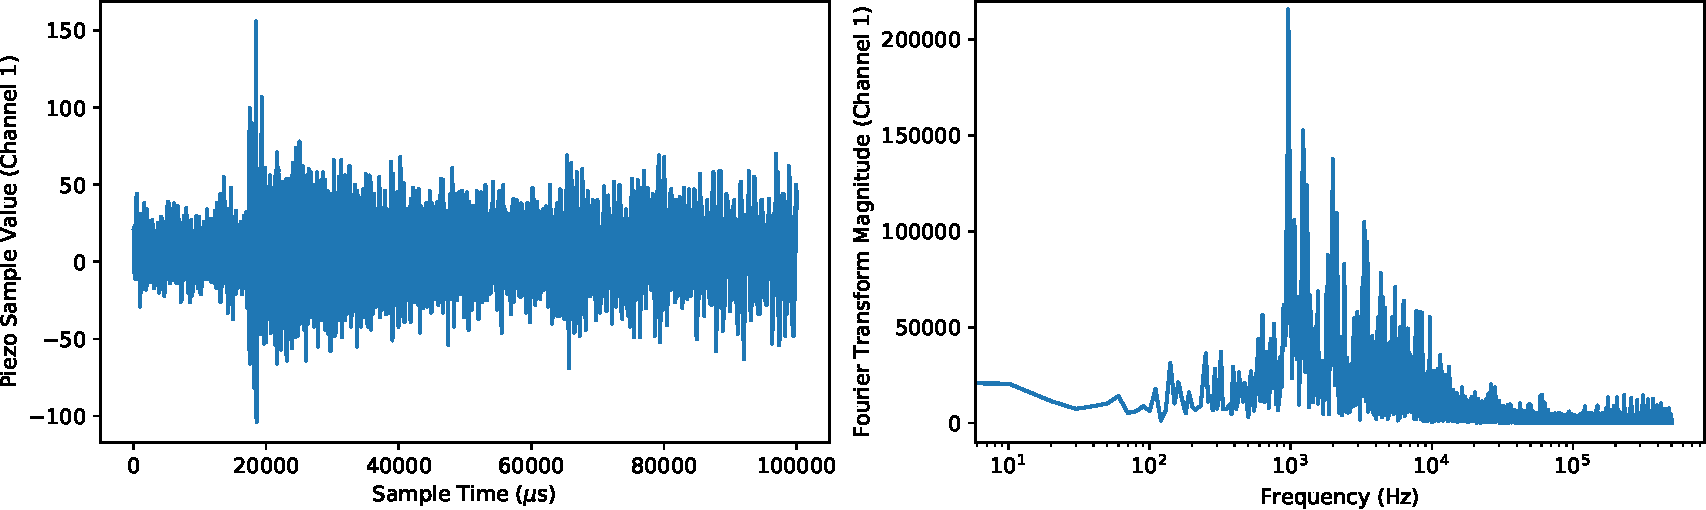
\includegraphics[width=0.95\textwidth]{audio_cropped}}}
    \qquad
    \subfloat{\fbox{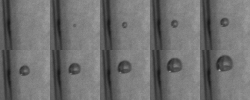
\includegraphics[width=0.35\textwidth]{image_grid}}}
    \caption{Examples of the audio and image data.}
\end{figure}

\subsubsection{Semi-Supervised Learning}

To better handle impurities, I developed two novel semi-supervised learning techniques. The concept of both algorithms is to iteratively generate more accurate labels for a set of inaccurately labeled training data, permitting less overfitting and greater validation accuracy than simple regularization would allow.

\begin{enumerate}
    \item Iterative Clustering is inspired by unsupervised clustering algorithms, and takes advantage of the ``confidence'' of the neural network's predictions (that is, how close the predictions are to 0 or 1).
    
    First, a neural network is trained on a labeled set. After 30 epochs, it runs predictions on the unlabeled set. As the network trains, the confidence of these predictions increases. When $p < t$ or $p > 1 - t$ for a given prediction $p$ and a (small) confidence threshold $t$, the example is labeled correspondingly and added to the labeled set.

    It is hypothesized that accuracy will gradually \textit{improve} as the neural network's most confident predictions are fed back into the network as newly labeled training data.

    \item Gravitational Differentiation is an analog alternative to Iterative Clustering. Using a novel piecewise exponential function for calculating final-layer derivatives, called $\mathrm{GravDiff}(p, \psi, g)$, unlabeled examples are caused to "gravitate" toward more accurate predictions based on the confidence of the neural network's predictions.

    The function is a transformation of the hyperbolic tangent that flattens the central range and comparatively exaggerates the asymptote on either side, defined as follows:
    \begin{center}
        $\mathrm{GravDiff}(p, \psi, g) = g \cdot \mathrm{sgn}(p) \cdot \lvert \mathrm{tanh}(2p - 1) \rvert ^ \psi$
    \end{center}
    where $p$ is the network's prediction, $\psi$ determines the rate at which the output approaches 0 as the confidence of the prediction decreases, and $g$ is the learning rate multiplier. The output is the final-layer gradient to be used in backpropagation.
\end{enumerate}

\subsection{Resolving Unpredictable Photon Dynamics (DEAP-3600)}

In DEAP-3600, the key challenge is the aforementioned unpredictable photon dynamics. The major source of background radiation is ``neck alphas'', which strike atoms in the gas filling the neck above the spherical detector body; because of the unpredictable direction of photon emission, it is non-trivial to calculate the position of these events.

Because of the inherently spatial nature of this problem, I hypothesized it would be important to most effectively process the spherical arrangement of PMTs in the DEAP-3600 detector. I evaluated three approaches to this problem (two of which are original), listed below. Techniques \ref{map_entry} and \ref{topological_entry} (Figure \ref{deap_methods}) take advantage of geometric and spatial patterns in PMT activations associated with neck alpha events, by extending the CNN concept for use in spherical and arbitrary topologies.

\begin{enumerate}
    \item I inputted photon counts from each PMT into a multi-layer perceptron.

    \item I developed and applied a Mercator-like cylindrical projection, which maps a sphere onto a rectangle. Cubic spline interpolation was used to map latitude lines on the hexagonal lattice (which vary in length) to equal-length rows on the rectangular image. Once again, photon counts were used as input data. \label{map_entry}

    \item I developed a new type of CNN, called a topological CNN. Rather than a 2D image of square pixels, kernels convolve over an arbitrary topology. \label{topological_entry}
    
    While a conventional convolutional layer downscales a rectangular image to a smaller rectangular image by multiplying square regions by a set of corresponding weights, a topological CNN (as applied to this problem) downscales the approximately spherical hexagonal mesh to a smaller but topologically equivalent hexagonal mesh.
\end{enumerate}

\begin{figure}[ht]
    \centering
    \fbox{
\includegraphics[width=0.425\textwidth]{map_projection}}
    \qquad
    \fbox{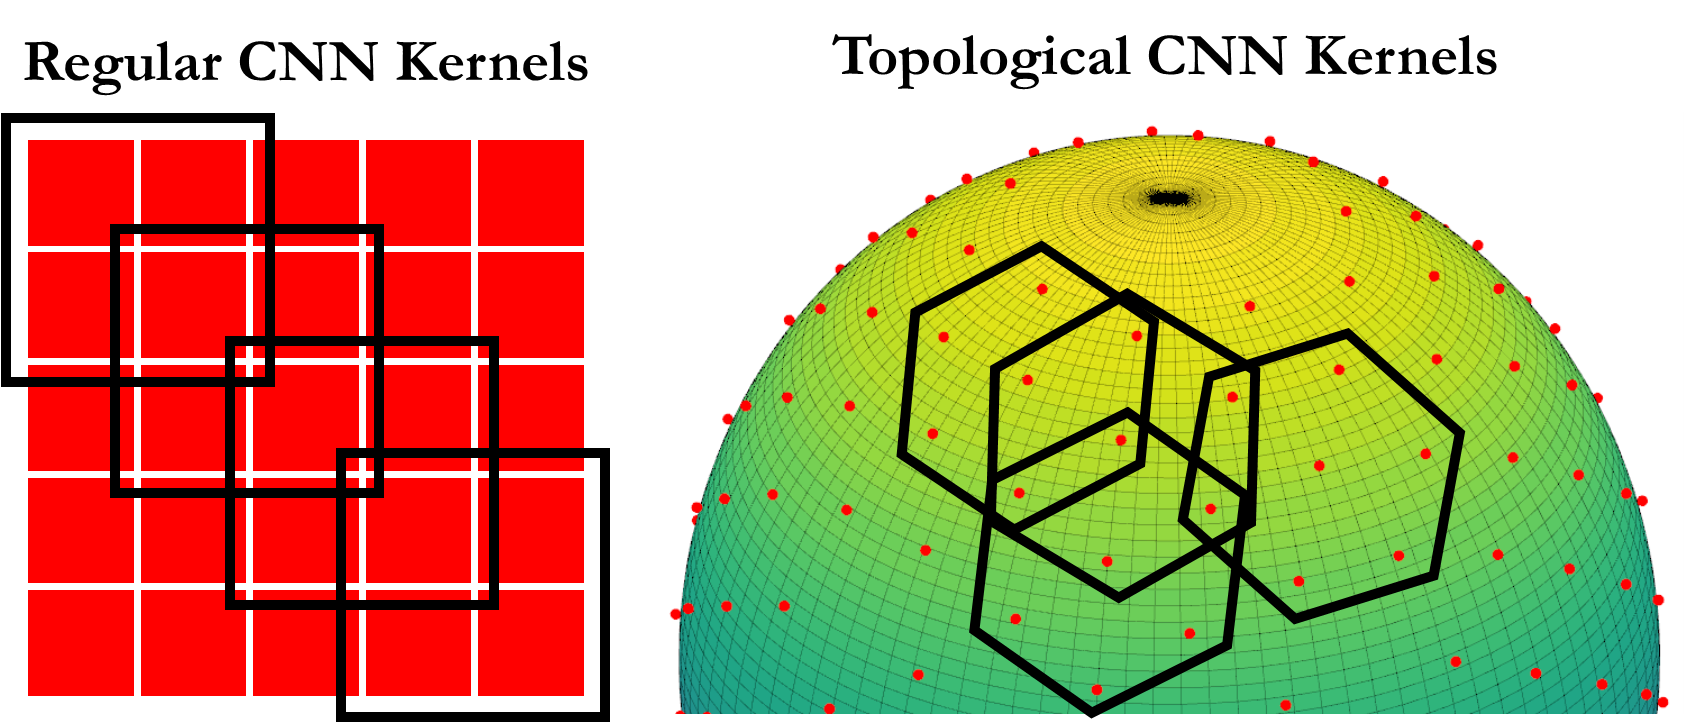
\includegraphics[width=0.475\textwidth]{topological}}
    \caption{\label{deap_methods} Diagrams of the cylindrical projection (left) and topological CNN (right) systems.}
\end{figure}

\subsection{Statistical Practices}

Models were optimized using grid searches, in which every configuration within a hyperparameter space is trained and evaluated. The best-performing technique and hyperparameters were selected based on repeated random sub-sampling of validation sets.

Finally, the best-performing model was retrained on a newly selected training set, and a test set was used to verify its performance. In DEAP-3600, two test sets were used: one consisting of simulated data, and another consisting of 30 examples collected from the real-world detector (neutron calibration data, and background radiation).

\section{Results}

\subsection{PICO-60}

As seen in Figure \ref{pico_final_results}, the banded Fourier transform format was the most effective of the supervised learning models (including the previous study), achieving 97.3\% validation accuracy. The image data was shown to contain no useful information, reaching only 63.0\% accuracy.

Semi-supervised learning produced better accuracy than supervised learning. Gravitational differentiation was the best overall model, achieving 99.7\% accuracy on validation data and 98.3\% on test data. This confirms my hypothesis; it is indeed beneficial to train on the neural network's most confident predictions.

\begin{figure}[ht]
    \centering
    \fbox{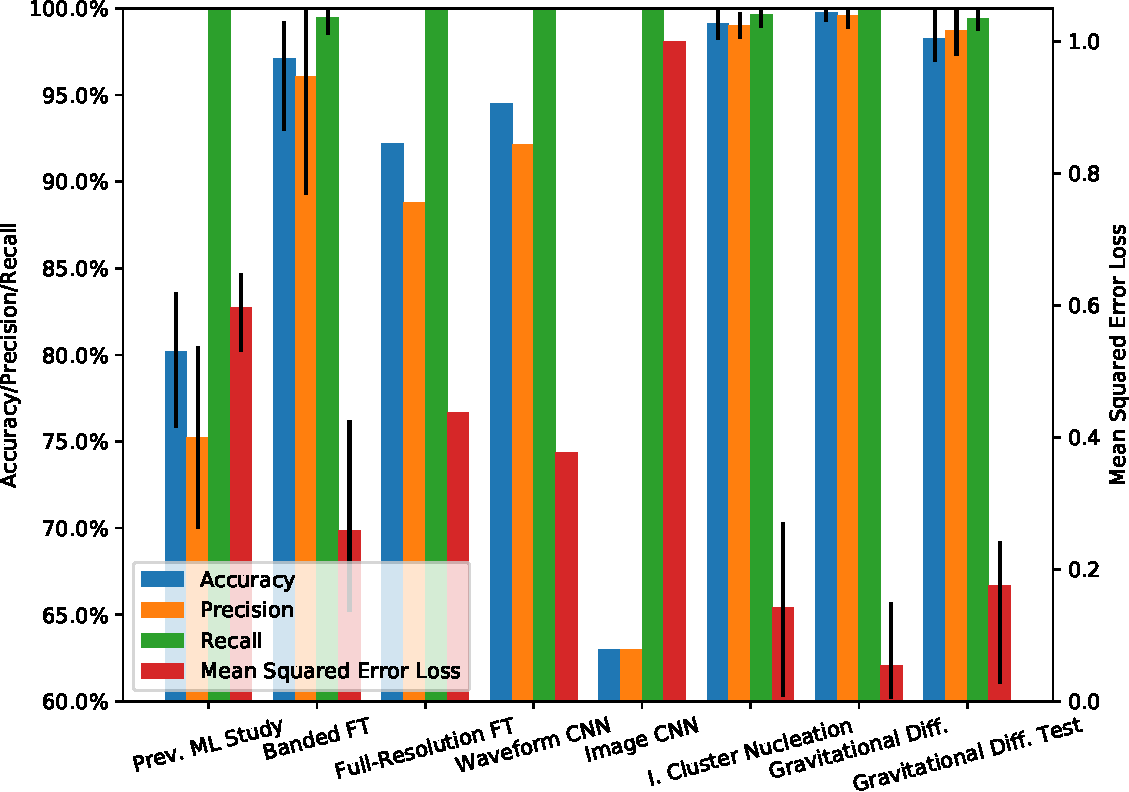
\includegraphics[width=0.85\textwidth]{pico_final_results}}
    \caption{\label{pico_final_results} Validation accuracy, precision, recall, and loss for each technique in PICO-60. Error bars represent the 8th and 92nd percentiles.}
\end{figure}

\subsection{DEAP-3600}

I evaluated three algorithms for resolution of the unpredictable photon dynamics present in DEAP-3600. Two of the algorithms are original. The three algorithms I developed were evaluated based on:

\begin{itemize}
    \item Identification of neck alphas with a minimum of 99.6\% precision (the same as the previously developed conventional classifier).
    \item Reduction in the rate of false positives (simulated WIMP events misidentified as neck alphas) compared to the 91.0\% result achieved with a conventional classifier.
\end{itemize}

All techniques were validated on simulated data. Both the dense neural network and topological CNN techniques were unsuccessful; they produced higher false positive rates than the conventional classifier, meaning that they misclassified more WIMPs as alpha particles.

However, as seen in Figure \ref{deap_final_results}, the cylindrical projection method retained a 99.6\% neck alpha identification rate, and also successfully \textit{reduced} the false positive rate from 91.0\% to 75.7\%.

This successful network model was further tested on the limited amount of available real-world experimental data. It removed 73.9\% of WIMP-like (neutron calibration) events, which is in line with the 75.7\% obtained on simulated data.

However, only 91.2\% of background events (expected to be neck alphas) were removed, below the 99.6\% reached on simulated data. This indicates one of three possibilities:

\begin{enumerate}
    \item The simulation is not an accurate representation of the real-world detector (some physical dynamic has not been simulated), and thus the network did not generalize.
    \item There is WIMP dark matter present in the set of background events.
    \item There is an unanticipated form of background radiation present.
\end{enumerate}

\begin{figure}[ht]
    \centering
    \definecolor{lightcyan}{rgb}{0.8, 1, 1}
    \begin{tabular}[b]{|l|l|l|l|}
        \hline
        \rowcolor{lightcyan}
        Technique & Data Source & Background & False Positive Rate \\
        \rowcolor{lightcyan}
        & & Removal Rate & (WIMP Misclassifications) \\
        \hline
        Conventional Classifier & Simulation (Val.) & 99.6\% & 91.0\% \\
        \hline
        Dense Neural Network & Simulation (Val.) & 100\% & 100\% \\
        \hline
        Cylindrical Projection & Simulation (Val.) & 99.9\% & 76.7\% \\
        \hline
        Topological CNN & Simulation (Val.) & 99.9\% & 93.0\% \\
        \hline
        Cylindrical Projection & Simulation (Test) & 99.6\% & 75.7\% \\
        \hline
        Cylindrical Projection & Real-World & 91.2\% & 73.9\% \\
        \hline
    \end{tabular}
    \caption{\label{deap_final_results} Average background and WIMP/neutron removal rates for the highest-accuracy hyperparameter configuration of each technique in DEAP-3600.}
\end{figure}

\section{Conclusion}

These results confirm that I met my goals on both the PICO-60 and DEAP-3600 experiments.

On PICO-60, the new semi-supervised learning algorithms performed extremely well, exceeding 98\% accuracy while permitting impure calibration data and requiring little manual analysis or optimization.

On DEAP-3600, my cylindrical projection, combined with a 2D CNN, performed better than the conventional classifier on simulated data, reducing the WIMP misclassification rate from 91.0\% to 75.7\% while matching the conventional classifier's 99.6\% background removal rate.

The predictions made on real-world data demonstrate clear potential. Differences between the simulated and real-world data provide potentially useful diagnostic information on the DEAP-3600 simulation (assuming that WIMPs are not present).

Fundamentally, the problems I have solved are not specific to PICO-60 and DEAP-3600; they are common across many dark matter detection experiments. Thus, my algorithms are broadly applicable, and demonstrate promise in the field as a whole.

\section{Acknowledgements}

Many thanks to Dr.~Nigel~Smith, Dr.~Ken~Clark, Dr.~Carsten~Krauss, Dr.~Scott~Fallows, Dr.~Eric~V\'azquez-J\'auregui, and Dr.~Pierre~Gorel for introducing me to PICO-60 and DEAP-3600, and generously providing access to data for training.

\section{References}

\printbibliography[heading=none]

\pagebreak

\section{Bibliography}

\begin{itemize}
    \item All programming for this study was done in Python 3 \cite{python}.
    \item Keras \cite{keras}, running on a TensorFlow \cite{tensorflow} backend, was used for all machine learning tasks.
    \item NumPy \cite{numpy} and SciPy \cite{scipy} were used for linear algebra and signal processing.
    \item ROOT \cite{root}, scikit-image \cite{scikit-image}, and scikit-learn \cite{scikit-learn} were used for data loading and storage.
    \item Matplotlib \cite{matplotlib} was used for data visualization.
\end{itemize}

\end{document}